\documentclass{standalone}
\usepackage{tikz}
\usetikzlibrary{patterns, positioning}


\begin{document}
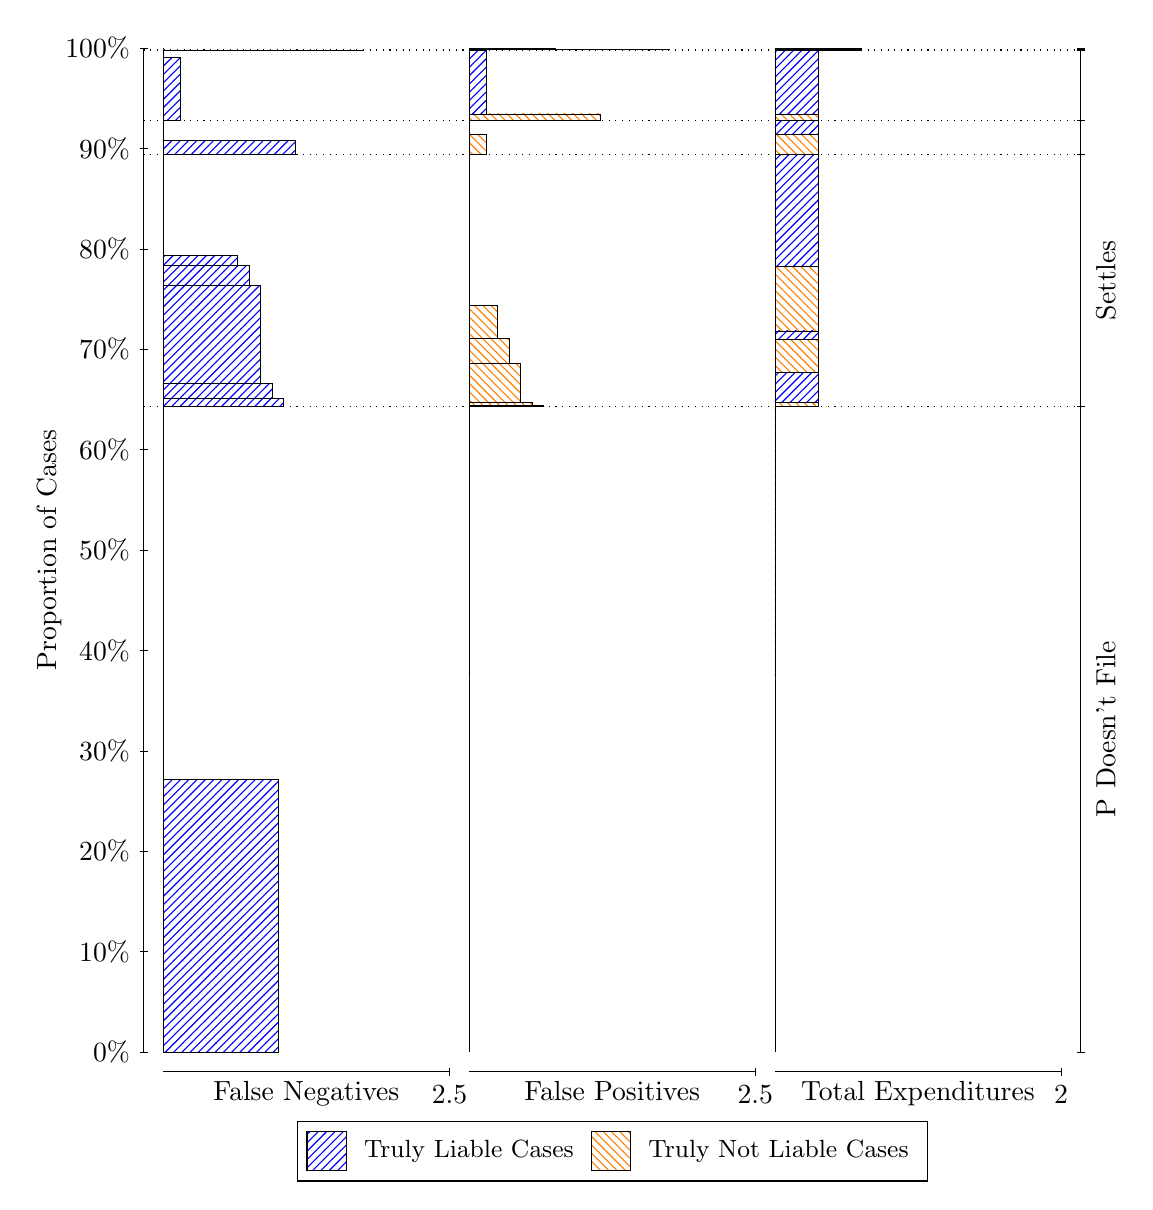
\begin{tikzpicture}
\draw[black, very thin] (1.5,1.75) -- (1.5,14.5);
\node[rotate=90, text=black, anchor=center] at (0.3, 8.125) {Proportion of Cases};
\draw[black, very thin] (1.45,1.75) -- (1.55,1.75);
\node[text=black, anchor=east] at (1.45, 1.75) {0\%};
\draw[black, very thin] (1.45,3.025) -- (1.55,3.025);
\node[text=black, anchor=east] at (1.45, 3.025) {10\%};
\draw[black, very thin] (1.45,4.3) -- (1.55,4.3);
\node[text=black, anchor=east] at (1.45, 4.3) {20\%};
\draw[black, very thin] (1.45,5.575) -- (1.55,5.575);
\node[text=black, anchor=east] at (1.45, 5.575) {30\%};
\draw[black, very thin] (1.45,6.85) -- (1.55,6.85);
\node[text=black, anchor=east] at (1.45, 6.85) {40\%};
\draw[black, very thin] (1.45,8.125) -- (1.55,8.125);
\node[text=black, anchor=east] at (1.45, 8.125) {50\%};
\draw[black, very thin] (1.45,9.4) -- (1.55,9.4);
\node[text=black, anchor=east] at (1.45, 9.4) {60\%};
\draw[black, very thin] (1.45,10.675) -- (1.55,10.675);
\node[text=black, anchor=east] at (1.45, 10.675) {70\%};
\draw[black, very thin] (1.45,11.95) -- (1.55,11.95);
\node[text=black, anchor=east] at (1.45, 11.95) {80\%};
\draw[black, very thin] (1.45,13.225) -- (1.55,13.225);
\node[text=black, anchor=east] at (1.45, 13.225) {90\%};
\draw[black, very thin] (1.45,14.5) -- (1.55,14.5);
\node[text=black, anchor=east] at (1.45, 14.5) {100\%};

\draw[black, very thin] (13.4,1.75) -- (13.4,14.5);
\draw[black, very thin] (13.35,1.75) -- (13.45,1.75);
\node[anchor=west] at (13.35, 1.75) {};
\draw[black, very thin] (13.35,9.95) -- (13.45,9.95);
\node[anchor=west] at (13.35, 9.95) {};
\draw[black, very thin] (13.35,13.152) -- (13.45,13.152);
\node[anchor=west] at (13.35, 13.152) {};
\draw[black, very thin] (13.35,13.577) -- (13.45,13.577);
\node[anchor=west] at (13.35, 13.577) {};
\draw[black, very thin] (13.35,14.469) -- (13.45,14.469);
\node[anchor=west] at (13.35, 14.469) {};
\draw[black, very thin] (13.35,14.479) -- (13.45,14.479);
\node[anchor=west] at (13.35, 14.479) {};
\draw[black, very thin] (13.35,14.5) -- (13.45,14.5);
\node[anchor=west] at (13.35, 14.5) {};

\draw[black, very thin, pattern color=blue, pattern=north east lines] (1.75,1.75) rectangle (3.2033,5.2097);
\draw[black, very thin, pattern color=orange, pattern=north west lines] (1.75,5.2097) rectangle (1.75,9.95);
\draw[black, very thin, pattern color=blue, pattern=north east lines] (1.75,9.95) rectangle (3.276,10.054);
\draw[black, very thin, pattern color=blue, pattern=north east lines] (1.75,10.054) rectangle (3.1307,10.238);
\draw[black, very thin, pattern color=blue, pattern=north east lines] (1.75,10.238) rectangle (2.9853,11.482);
\draw[black, very thin, pattern color=blue, pattern=north east lines] (1.75,11.482) rectangle (2.84,11.742);
\draw[black, very thin, pattern color=blue, pattern=north east lines] (1.75,11.742) rectangle (2.6947,11.866);
\draw[black, very thin, pattern color=orange, pattern=north west lines] (1.75,11.866) rectangle (1.75,13.152);
\draw[black, very thin, pattern color=blue, pattern=north east lines] (1.75,13.152) rectangle (3.4213,13.325);
\draw[black, very thin, pattern color=orange, pattern=north west lines] (1.75,13.325) rectangle (1.75,13.577);
\draw[black, very thin, pattern color=blue, pattern=north east lines] (1.75,13.577) rectangle (1.968,14.381);
\draw[black, very thin, pattern color=orange, pattern=north west lines] (1.75,14.381) rectangle (1.75,14.469);
\draw[black, very thin, pattern color=blue, pattern=north east lines] (1.75,14.469) rectangle (4.2933,14.474);
\draw[black, very thin, pattern color=orange, pattern=north west lines] (1.75,14.474) rectangle (1.75,14.479);
\draw[black, very thin, pattern color=orange, pattern=north west lines] (1.75,14.479) rectangle (1.75,14.484);
\draw[black, very thin, pattern color=blue, pattern=north east lines] (1.75,14.484) rectangle (1.75,14.5);
\draw[black, very thin, pattern color=orange, pattern=north west lines] (5.6333,1.75) rectangle (5.6333,6.4903);
\draw[black, very thin, pattern color=blue, pattern=north east lines] (5.6333,6.4903) rectangle (5.6333,9.95);
\draw[black, very thin, pattern color=orange, pattern=north west lines] (5.6333,9.95) rectangle (6.578,9.9601);
\draw[black, very thin, pattern color=orange, pattern=north west lines] (5.6333,9.9601) rectangle (6.4327,9.9948);
\draw[black, very thin, pattern color=orange, pattern=north west lines] (5.6333,9.9948) rectangle (6.2873,10.499);
\draw[black, very thin, pattern color=orange, pattern=north west lines] (5.6333,10.499) rectangle (6.142,10.811);
\draw[black, very thin, pattern color=orange, pattern=north west lines] (5.6333,10.811) rectangle (5.9967,11.235);
\draw[black, very thin, pattern color=blue, pattern=north east lines] (5.6333,11.235) rectangle (5.6333,13.152);
\draw[black, very thin, pattern color=orange, pattern=north west lines] (5.6333,13.152) rectangle (5.8513,13.403);
\draw[black, very thin, pattern color=blue, pattern=north east lines] (5.6333,13.403) rectangle (5.6333,13.577);
\draw[black, very thin, pattern color=orange, pattern=north west lines] (5.6333,13.577) rectangle (7.3047,13.664);
\draw[black, very thin, pattern color=blue, pattern=north east lines] (5.6333,13.664) rectangle (5.8513,14.469);
\draw[black, very thin, pattern color=orange, pattern=north west lines] (5.6333,14.469) rectangle (5.6333,14.474);
\draw[black, very thin, pattern color=blue, pattern=north east lines] (5.6333,14.474) rectangle (5.6333,14.479);
\draw[black, very thin, pattern color=orange, pattern=north west lines] (5.6333,14.479) rectangle (8.1767,14.484);
\draw[black, very thin, pattern color=blue, pattern=north east lines] (5.6333,14.484) rectangle (6.7233,14.5);
\draw[black, very thin, pattern color=orange, pattern=north west lines] (9.5167,1.75) rectangle (9.5167,6.4903);
\draw[black, very thin, pattern color=blue, pattern=north east lines] (9.5167,6.4903) rectangle (9.5167,9.95);
\draw[black, very thin, pattern color=orange, pattern=north west lines] (9.5167,9.95) rectangle (10.062,9.9948);
\draw[black, very thin, pattern color=blue, pattern=north east lines] (9.5167,9.9948) rectangle (10.062,10.379);
\draw[black, very thin, pattern color=orange, pattern=north west lines] (9.5167,10.379) rectangle (10.062,10.804);
\draw[black, very thin, pattern color=blue, pattern=north east lines] (9.5167,10.804) rectangle (10.062,10.908);
\draw[black, very thin, pattern color=orange, pattern=north west lines] (9.5167,10.908) rectangle (10.062,11.724);
\draw[black, very thin, pattern color=blue, pattern=north east lines] (9.5167,11.724) rectangle (10.062,13.152);
\draw[black, very thin, pattern color=orange, pattern=north west lines] (9.5167,13.152) rectangle (10.062,13.403);
\draw[black, very thin, pattern color=blue, pattern=north east lines] (9.5167,13.403) rectangle (10.062,13.577);
\draw[black, very thin, pattern color=orange, pattern=north west lines] (9.5167,13.577) rectangle (10.062,13.664);
\draw[black, very thin, pattern color=blue, pattern=north east lines] (9.5167,13.664) rectangle (10.062,14.469);
\draw[black, very thin, pattern color=orange, pattern=north west lines] (9.5167,14.469) rectangle (10.607,14.474);
\draw[black, very thin, pattern color=blue, pattern=north east lines] (9.5167,14.474) rectangle (10.607,14.479);
\draw[black, very thin, pattern color=orange, pattern=north west lines] (9.5167,14.479) rectangle (10.607,14.484);
\draw[black, very thin, pattern color=blue, pattern=north east lines] (9.5167,14.484) rectangle (10.607,14.5);
\draw[black, dotted] (1.5,9.95) -- (13.4,9.95);
\draw[black, dotted] (1.5,13.152) -- (13.4,13.152);
\draw[black, dotted] (1.5,13.577) -- (13.4,13.577);
\draw[black, dotted] (1.5,14.469) -- (13.4,14.469);
\draw[black, dotted] (1.5,14.479) -- (13.4,14.479);
\draw[black, very thin] (1.75,1.5) -- (5.3833,1.5);
\node[text=black, anchor=north] at (3.5667, 1.5) {False Negatives};
\draw[black, very thin] (5.3833,1.45) -- (5.3833,1.55);
\node[text=black, anchor=north] at (5.3833, 1.45) {2.5};

\draw[black, very thin] (5.6333,1.5) -- (9.2667,1.5);
\node[text=black, anchor=north] at (7.45, 1.5) {False Positives};
\draw[black, very thin] (9.2667,1.45) -- (9.2667,1.55);
\node[text=black, anchor=north] at (9.2667, 1.45) {2.5};

\draw[black, very thin] (9.5167,1.5) -- (13.15,1.5);
\node[text=black, anchor=north] at (11.333, 1.5) {Total Expenditures};
\draw[black, very thin] (13.15,1.45) -- (13.15,1.55);
\node[text=black, anchor=north] at (13.15, 1.45) {2};

\node[text=black, centered, rotate=90] at (13.72, 5.85) {P Doesn't File};
\node[text=black, centered, rotate=90] at (13.72, 11.551) {Settles};





\draw (7.449999999999999,1.5) node[draw=none] (baseCoordinate) {};
\begin{scope}[align=center]
        \matrix[scale=0.5, draw=black, below=0.5cm of baseCoordinate, nodes={draw}, column sep=0.1cm]{
            \node[rectangle, draw, minimum width=0.5cm, minimum height=0.5cm, pattern color=blue, pattern=north east lines] {}; &
            \node[draw=none, font=\small, text=black] (B) {Truly Liable Cases}; &
            \node[rectangle, draw, minimum width=0.5cm, minimum height=0.5cm, pattern color=orange, pattern=north west lines] {}; &
            \node[draw=none, font=\small, text=black] (B) {Truly Not Liable Cases}; \\
            };
\end{scope}

\end{tikzpicture}
\end{document}